% EEE3096S Practical 2: Memory-Mapped I/O and Hardware SPI
% Build: pdflatex prac_02_lxxtri004_shrgil004.tex  (run twice for references)
%
% Anything still to be measured is wrapped in \bench{} and renders red, so an
% unfilled slot cannot be mistaken for a result. The report is not ready to
% submit while any red remains.

\documentclass[conference]{IEEEtran}

\usepackage{graphicx}
\usepackage{amsmath}
\usepackage{booktabs}
\usepackage{xcolor}
\usepackage{float}
\usepackage[hidelinks]{hyperref}
\usepackage{tikz}
\usetikzlibrary{automata, positioning, arrows.meta, fit}

\newcommand{\bench}[1]{\textcolor{red}{\textbf{[BENCH: #1]}}}

% Figure slot for a capture that does not exist yet. Drop the file into
% figures/ under the name given and it appears with no edit here.
\newcommand{\scopefig}[3]{%
  \begin{figure}[htbp]
  \centering
  \IfFileExists{figures/#1}{%
    \includegraphics[width=\linewidth]{figures/#1}%
  }{%
    \fbox{\parbox[c][40mm][c]{0.92\linewidth}{\centering
      \textcolor{red}{\textbf{[BENCH] figures/#1 not captured yet}}}}%
  }
  \caption{#3}
  \label{fig:#2}
  \end{figure}%
}

% ============================================================================
% BENCH MEASUREMENTS - the only file that needs editing after the lab session.
%
% Each entry below is a slot. Replace the \bench{...} with the value measured,
% keeping the braces. Anything still holding a \bench{...} renders red in the
% PDF, so the report is finished exactly when nothing here is red any more.
%
% Do not put a value here that was not actually measured.
% ============================================================================

% --- Section 2: wiring confirmed with a meter -------------------------------
% One or two sentences: which pins were checked, what the anchor pins (EEPROM
% VCC to 3V3, VSS to GND) did, and whether the README's mapping held.
\newcommand{\mWiring}{\bench{continuity check result}}

% --- Section 3: the SCK and MOSI capture ------------------------------------
\newcommand{\mSckPeriod}{\bench{SCK period, e.g. 4.02 us}}
\newcommand{\mSckFreq}{\bench{1/period, e.g. 248.8 kHz}}
\newcommand{\mSckError}{\bench{percent error against 250 kHz}}
\newcommand{\mClockIdle}{\bench{idle state of SCK, high or low}}
\newcommand{\mClockCycles}{\bench{clock cycles counted in the capture}}

% Bit sequence read off the screen, MSB first, and the value it reconstructs.
% Read this from the waveform, not from the source.
\newcommand{\mDecodedBits}{\bench{eight bits in order}}
\newcommand{\mDecodedValue}{\bench{value they give}}
\newcommand{\mSampleEdge}{\bench{which edge the device samples on}}

% --- Section 4: the EEPROM ---------------------------------------------------
% How the address width was confirmed on the bench, including what the status
% register showed after a deliberate short write if that was tried.
\newcommand{\mAddressWidth}{\bench{how the two-byte address was confirmed}}

\newcommand{\mStatusBefore}{\bench{eeprom\_status\_before}}
\newcommand{\mStatusAfter}{\bench{eeprom\_status\_after}}
\newcommand{\mWriteWait}{\bench{eeprom\_write\_wait\_ms}}
\newcommand{\mValueWritten}{\bench{value written}}
\newcommand{\mValueRead}{\bench{value read back}}
\newcommand{\mVerifyResult}{\bench{passed or failed}}
\newcommand{\mPulseCount}{\bench{clock pulses while CS is low}}

% What was written, what the reset was, what came back afterwards.
\newcommand{\mPersistence}{\bench{persistence test result}}

% --- Section 5: the fault ----------------------------------------------------
% The four table columns. Keep each to a phrase; the narrative goes below.
\newcommand{\mFaultExpected}{\bench{expected}}
\newcommand{\mFaultObserved}{\bench{observed}}
\newcommand{\mFaultCause}{\bench{register and field}}
\newcommand{\mFaultCorrection}{\bench{correction}}

% The diagnosis in prose: the first meaningful difference between the two
% captures, and why the corrected configuration now satisfies the device
% electrically. This is where the marks are.
\newcommand{\mFaultNarrative}{\bench{diagnosis: first difference, why the
correction works electrically}}

% --- Section 6: the state machine --------------------------------------------
% What PC13 did in each mode, with ee_use_fsm at 1 and at 0.
\newcommand{\mHeartbeat}{\bench{heartbeat under the FSM versus the blocking path}}

% One complete run through the state machine.
\newcommand{\mFsmResult}{\bench{one write, read and verify result via the FSM}}


\begin{document}

\title{Memory-Mapped I/O and Hardware SPI:\\Building and Debugging an EEPROM Driver}

\author{\IEEEauthorblockN{Tri Tac Le}
\IEEEauthorblockA{LXXTRI004\\Department of Electrical Engineering\\University of Cape Town}
\and
\IEEEauthorblockN{Gil Sharon}
\IEEEauthorblockA{SHRGIL004\\Department of Electrical Engineering\\University of Cape Town}}

\maketitle

\begin{abstract}
Complete source code for this practical is in the group repository at
\url{https://github.com/TriTacLe/EEE3096S-prac2}. The firmware builds with
\texttt{make} in \texttt{Practical2\_A}, and \texttt{make RUN\_TASK=n} selects
the task under test.
\end{abstract}

\section{Memory-Mapped GPIO}

\subsection{Addresses and offsets}

Peripheral registers occupy ordinary addresses in the processor's address
space, so each one is reached as $A_{\text{register}} = B + O$ for a peripheral
base $B$ and a register offset $O$. Table~\ref{tab:addresses} gives the values
used for Task 1 and the document each came from.

\begin{table}[htbp]
\caption{Task 1 register addresses}
\label{tab:addresses}
\centering
\begin{tabular}{llll}
\toprule
Register & Base & Offset & Source \\
\midrule
RCC\_AHBENR  & 0x40021000 & 0x14 & \cite{rm0091}, Table 1, \S7.4.6 \\
GPIOC\_MODER & 0x48000800 & 0x00 & \cite{rm0091}, Table 1, \S9.4.1 \\
GPIOC\_ODR   & 0x48000800 & 0x14 & \cite{rm0091}, \S9.4.6 \\
GPIOC\_BSRR  & 0x48000800 & 0x18 & \cite{rm0091}, \S9.4.7 \\
GPIOC\_BRR   & 0x48000800 & 0x28 & \cite{rm0091}, \S9.4.11 \\
\bottomrule
\end{tabular}
\end{table}

\subsection{Bit masks}

The port C peripheral clock is enabled by IOPCEN, bit 19 of RCC\_AHBENR
\cite{rm0091}. Without it the GPIO registers are not clocked: writes are
discarded and reads return zero, so the code appears to run correctly while the
pin never moves.

MODER holds two bits per pin, so PC13 occupies bits 27:26. The field is cleared
with a mask of \texttt{0x3 << 26} and then written with \texttt{0x1 << 26} for
general purpose output mode. Clearing before setting matters because the field
is not a single bit, and leaving the other 15 pins untouched requires a
read-modify-write rather than a plain store.

The toggle uses BSRR and BRR rather than a read-modify-write of ODR. Each of
those registers affects only the bits written to it, so the operation is a
single store and cannot lose a concurrent write to another pin on the same
port. This matters in Tasks 4 and 6, where PB12 carries the chip select on the
port that also drives the LEDs.

\subsection{The role of \texttt{volatile}}

A peripheral register can change independently of program flow, and reading or
writing one can itself cause an effect. Without \texttt{volatile} the compiler
is entitled to keep a previously read value in a core register, to reorder
accesses, or to discard a store whose result is never read. Any of those breaks
a hardware access: a status flag polled in a loop would be read once and the
loop would never terminate, and a write that starts a peripheral operation
would be optimised away because nothing in the C program reads it back.
Declaring the pointer \texttt{volatile} requires the compiler to perform every
access exactly as written.

\scopefig{task1-pc13.png}{task1}{PC13 output generated through memory-mapped
register writes only, with no HAL GPIO calls.}

\section{Hardware SPI Configuration}

\subsection{Configuration table}

\begin{table}[htbp]
\caption{SPI configuration, with the source of each field}
\label{tab:spiconfig}
\centering
\begin{tabular}{llp{2.4cm}}
\toprule
Item & Value & Source \\
\midrule
SPI peripheral    & SPI2         & \cite{f051ds}, Table 15 \\
Peripheral clock  & 8\,MHz       & \cite{rm0091}, \S7.2.2; Table 1 \\
PB13 alt.\ function & AF0, SPI2\_SCK  & \cite{f051ds}, Table 15 \\
PB14 alt.\ function & AF0, SPI2\_MISO & \cite{f051ds}, Table 15 \\
PB15 alt.\ function & AF0, SPI2\_MOSI & \cite{f051ds}, Table 15 \\
Clock divider     & BR = 100, $f_{\text{PCLK}}/32$ & \cite{rm0091}, \S27.7.1 \\
Predicted SCK     & 250\,kHz     & calculated below \\
CPOL              & 0            & \cite{cat25640}, SPI modes \\
CPHA              & 0            & \cite{cat25640}, SPI modes \\
Bit order         & MSB first    & \cite{cat25640}; CR1 LSBFIRST = 0 \\
\bottomrule
\end{tabular}
\end{table}

\subsection{Clock calculation}

\texttt{SystemClock\_Config()} selects HSI as the system clock with the PLL
disabled, and both the AHB and APB1 prescalers at unity. HSI is the internal
8\,MHz RC oscillator \cite{rm0091}, so

\[ f_{\text{SYSCLK}} = f_{\text{HCLK}} = f_{\text{PCLK1}} = 8\,\text{MHz}. \]

SPI2 is an APB1 peripheral \cite{rm0091}, so PCLK1 is its kernel clock. The BR
field divides by $2^{\text{BR}+1}$, and the target is 250\,kHz:

\[ \frac{8 \times 10^{6}}{250 \times 10^{3}} = 32 = 2^{5}
   \;\Rightarrow\; \text{BR} + 1 = 5 \;\Rightarrow\; \text{BR} = 4 = 100_2 \]

giving a predicted $f_{\text{SCK}}$ of exactly 250\,kHz. The divider was
derived from the clock tree rather than adjusted until the waveform looked
correct, and a compile-time assertion in \texttt{main.c} fails the build if the
configured divider and PCLK1 do not produce 250\,kHz.

\subsection{Alternate function selection}

Table 15 of \cite{f051ds} fixes SPI2\_SCK, SPI2\_MISO and SPI2\_MOSI to PB13,
PB14 and PB15 respectively, all on AF0. These assignments are fixed in silicon
and cannot be relocated, which is why the pin table given in the practical
handout cannot describe this device. The mapping confirmed on the board, and
used throughout, is PB12 chip select, PB13 SCK, PB14 EEPROM serial output and
PB15 EEPROM serial input. \mWiring

Three configuration choices are worth stating explicitly.

CR2 is written before the peripheral is enabled. It sets 8-bit frames and
FRXTH, which lowers the receive FIFO threshold so that RXNE is raised after
eight bits rather than sixteen \cite{rm0091}. The reset value of FRXTH is 0,
which would leave a single-byte transfer waiting for a second frame that never
arrives.

CR1 uses software slave management with the internal slave select held high.
Because the chip select is driven as an ordinary GPIO, nothing drives the
peripheral's NSS input; a master that observes NSS low clears MSTR and leaves
master mode of its own accord \cite{rm0091}, and the resulting symptom is the
absence of any clock rather than an incorrect one.

The chip select is driven high before MODER makes it an output, so the EEPROM
never observes an asserted chip select during initialisation.

\section{SPI Waveform}

\subsection{Group test byte}

With $n_1 = 4$ (LXXTRI004) and $n_2 = 4$ (SHRGIL004):

\begin{align*}
B &= \left[(n_1 \oplus n_2) + \text{0x3D}\right] \bmod 256 \\
  &= (0 + 61) \bmod 256 = \text{0x3D}
\end{align*}

Since both student numbers end in the same three digits the exclusive-or
vanishes. The result is neither 0x00 nor 0xFF, so the 0x5A substitution does
not apply and the group test byte is 0x3D, or $00111101_2$.

\subsection{Measured waveform}

\scopefig{task3-sck-mosi.png}{task3}{One complete byte transmitted with the
chip select held high. CH1 SCK, CH2 MOSI.}

Measured from the capture with cursors placed by hand: the clock idles
\mClockIdle, the capture contains \mClockCycles\ clock cycles, and the period
is $T_{\text{meas}} = \mSckPeriod$.

\[ f_{\text{meas}} = \frac{1}{T_{\text{meas}}}, \quad
   \%\,\text{err} = \frac{\left|f_{\text{meas}} - f_{\text{pred}}\right|}
                         {f_{\text{pred}}} \times 100 \]

This gives $f_{\text{meas}} = \mSckFreq$ against the predicted 250\,kHz, a
frequency error of \mSckError.

\subsection{Manual decoding}

Reading the eight data bits off the waveform in order, most significant first,
gives \mDecodedBits, which reconstructs \mDecodedValue. The device samples on
\mSampleEdge. The value is decoded from the capture rather than taken from the
source, so the waveform is the evidence that the configured bit order and
sampling edge are the ones actually generated.

\section{EEPROM Driver}

\subsection{Group address}

\[ A = (n_1 + 3n_2) \bmod 256 = (4 + 12) \bmod 256 = \text{0x10} \]

which lies well inside the 8192-byte array of the fitted device.

\subsection{Device identification}

The handout names a CAT25040, which is addressed with a single address byte.
The device fitted to this board accepts a 16-bit address and holds 8192 bytes,
which matches the CAT25640 \cite{cat25640}. Instructions that carry no address,
such as write-enable and read-status, behave identically on both parts, so the
distinction only appears once an address is sent: a write with too few address
bytes is discarded and the write enable latch remains set in the status
register afterwards. \mAddressWidth

\subsection{Transaction sequences}

Write-enable is issued as a complete transaction of its own. The write enable
latch is set on the rising edge of the chip select following the WREN opcode
\cite{cat25640}, so folding WREN into the beginning of the write transaction
would leave the latch unset and the subsequent write would be discarded.

A byte write consists of the WRITE opcode, two address bytes most significant
first, and the data byte, after which the chip select is raised. The internal
write cycle begins at that rising edge rather than at the final data bit, so no
status polling is meaningful until the transaction has closed.

A byte read consists of the READ opcode, the same two address bytes, and one
further byte clocked out to provide the eight edges on which the device shifts
its data back. SPI provides no independent read: the master owns the clock, so
receiving a byte always requires transmitting one, and the transmitted value is
ignored.

\subsection{Write completion}

Completion is determined from bit 0 of the status register. The bit is named
RDY but is asserted while the internal write cycle is in progress and clear
when the device is ready to accept commands \cite{cat25640}. Polling therefore
continues while the bit reads high. A fixed delay is not used anywhere in the
driver; the timeout of 50\,ms present in the code is an upper bound against a
device that never responds, against a datasheet maximum write cycle time of
5\,ms, and it is recorded separately from a verification failure.

The status register read \mStatusBefore\ before the write and \mStatusAfter\
after it. The write itself took \mWriteWait, against a datasheet maximum of
5\,ms. Writing \mValueWritten\ to address 0x10 and reading it back gave
\mValueRead, so verification \mVerifyResult.

\scopefig{task4-cs-sck.png}{task4}{A complete EEPROM transaction. CH1 chip
select, CH2 SCK, showing the number of clock pulses issued while the device is
selected.}

The capture shows \mPulseCount\ clock pulses issued while the device is
selected, which is consistent with one opcode byte, two address bytes and one
data byte at eight pulses each.

\subsection{Persistence}

\mPersistence

\section{Fault Diagnosis}

The repository contains a configuration fault applied only when the firmware is
built with \texttt{RUN\_TASK} set to 5. The same program built with
\texttt{RUN\_TASK} set to 4 runs without it, so the two differ by a single
configuration value and their measurements compare directly.

\subsection{Expected behaviour}

The comparison is only meaningful against a prediction made beforehand, so the
correct behaviour is stated here from the configuration of
Table~\ref{tab:spiconfig} rather than from what the board turned out to do.

With CPOL and CPHA both zero the clock idles low, the first edge of each bit
period is a rising edge, and the device samples on that first edge while the
master changes MOSI on the falling edge that follows. Data is transmitted most
significant bit first. Each byte is eight clock pulses, so a byte write of one
opcode, two address bytes and one data byte is 32 pulses issued while the chip
select is low, and the chip select frames the whole transaction without
returning high inside it. The period of each pulse is 4\,\textmu s at the
configured 250\,kHz.

Any departure from that list is the starting point of the diagnosis, and the
first departure in time is the one that matters: a difference later in a
transaction is usually a consequence of an earlier one rather than an
independent fault.

\begin{table}[htbp]
\caption{Fault diagnosis}
\label{tab:fault}
\centering
\begin{tabular}{p{1.6cm}p{1.6cm}p{1.6cm}p{1.6cm}}
\toprule
Expected & Observed & Cause & Correction \\
\midrule
\mFaultExpected & \mFaultObserved & \mFaultCause & \mFaultCorrection \\
\bottomrule
\end{tabular}
\end{table}

\mFaultNarrative

\scopefig{task5-faulty.png}{faulty}{The faulty case.}

\scopefig{task5-corrected.png}{corrected}{The same measurement after the
correction.}

\section{Non-Blocking FSM}

\subsection{State machine}

\begin{figure*}[htbp]
\centering
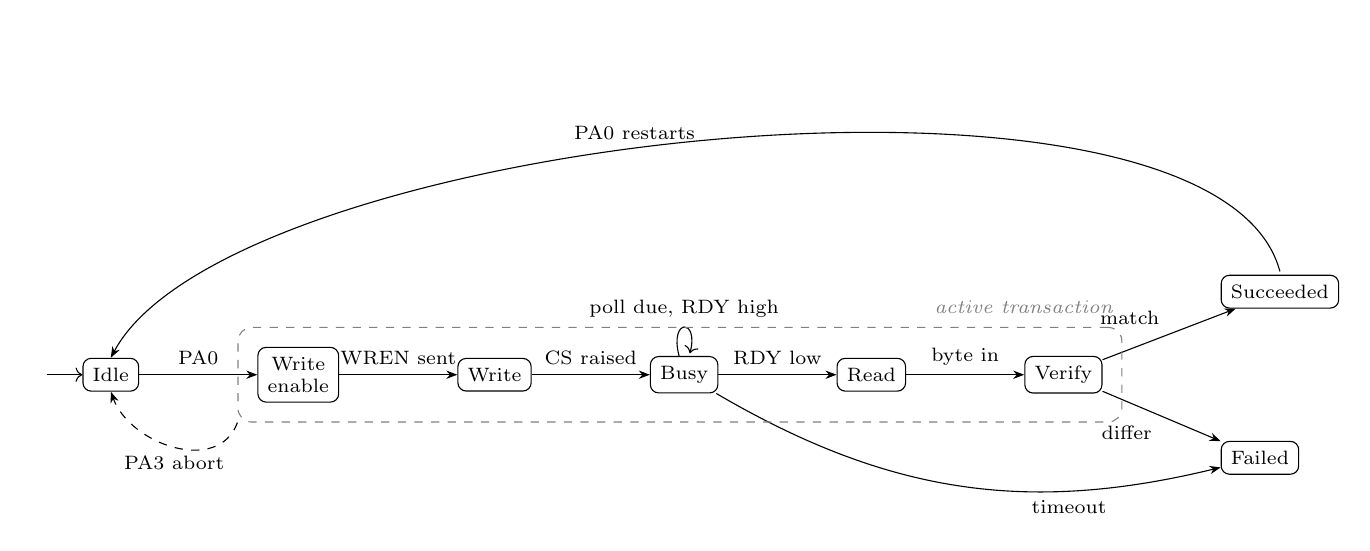
\begin{tikzpicture}[
  node distance = 14mm and 15mm,
  every state/.style = {draw, rectangle, rounded corners=3pt, inner sep=3.5pt,
                        minimum size=0pt, font=\scriptsize, align=center},
  every edge/.style = {draw, -{Stealth[length=4pt]}},
  auto, font=\scriptsize]

  \node[state, initial, initial text=] (idle)  {Idle};
  \node[state, right=of idle]   (wren)   {Write\\enable};
  \node[state, right=of wren]   (write)  {Write};
  \node[state, right=of write]  (busy)   {Busy};
  \node[state, right=of busy]   (read)   {Read};
  \node[state, right=of read]   (verify) {Verify};
  \node[state, above right=6mm and 15mm of verify] (ok)  {Succeeded};
  \node[state, below right=6mm and 15mm of verify] (bad) {Failed};

  \path (idle)   edge node {PA0} (wren)
        (wren)   edge node {WREN sent} (write)
        (write)  edge node {CS raised} (busy)
        (busy)   edge node {RDY low} (read)
        (read)   edge node {byte in} (verify)
        (verify) edge node {match} (ok)
        (verify) edge node[swap] {differ} (bad);

  \path (busy) edge [loop above] node {poll due, RDY high} (busy);
  \path (busy) edge [bend right=22] node[swap, pos=0.72] {timeout} (bad);

  % Both terminal states restart on PA0. One edge from the pair, routed over
  % the top, so it never crosses the abort path below.
  \node[fit=(ok)(bad), inner sep=1pt] (done) {};
  \draw[-{Stealth[length=4pt]}]
        (done.north) to[out=105, in=62, looseness=0.55]
        node[above, pos=0.55, font=\scriptsize] {PA0 restarts} (idle.north);

  % One abort boundary rather than five crossing edges, routed underneath.
  \node[draw, dashed, gray, rounded corners=5pt,
        fit=(wren)(write)(busy)(read)(verify), inner sep=7pt] (active) {};
  \node[gray, font=\scriptsize\itshape, above=0.5mm of active.north east,
        anchor=south east] {active transaction};
  \draw[dashed, -{Stealth[length=4pt]}]
        (active.south west) to[out=250, in=290, looseness=1.1]
        node[below, pos=0.5, font=\scriptsize] {PA3 abort} (idle.south);
\end{tikzpicture}
\caption{State diagram for the EEPROM transaction. PA3 returns the machine to
Idle from any state inside the dashed boundary. The self-loop on Busy is the
non-blocking wait: it is taken once per poll interval and returns immediately
rather than waiting inside the state.}
\label{fig:fsm}
\end{figure*}

The machine has eight states: idle, write-enable, write, busy, read, verify,
succeeded and failed. Write-enable and write are distinct states because the
write enable latch is set on the rising edge of the chip select after the WREN
opcode, so the two cannot share a transaction. Verify is separate from read so
that the comparison appears as a transition, making the success and failure
paths explicit.

\subsection{Transition logic}

A press of PA0 moves the machine out of idle. Each subsequent call performs one
step and returns: the write-enable transaction, then the write transaction,
after which the elapsed-time reference and the next status poll time are
recorded and the machine enters the busy state.

The busy state performs no waiting. On each call it compares the current tick
against the stored next-poll time and returns immediately unless a poll is due.
When one is due it performs a single status read and either advances to the
read state, remains busy, or fails on timeout. At a 1\,ms poll interval a
typical 5\,ms write costs approximately five status transactions while the main
loop continues to run.

PA3 returns the machine to idle from any active state. Every transaction raises
the chip select before the state advances, so an abort cannot leave the bus
with the chip select asserted. An abort during the busy state does not stop the
device: its internal write cycle began when the chip select rose and completes
regardless, so the abort abandons the host transaction rather than the
device's.

\subsection{Why it is non-blocking}

The blocking implementation of Task 4 remains available at runtime for
comparison, selected by the \texttt{ee\_use\_fsm} variable. In both modes PC13
continues to toggle as a heartbeat. In the blocking path the heartbeat stops
for the duration of the write cycle because the processor is inside the status
polling loop; under the state machine it continues without interruption, and
PA3 remains responsive throughout.

\mHeartbeat\ \mFsmResult

\begin{thebibliography}{9}

\bibitem{rm0091}
STMicroelectronics, \emph{RM0091 Reference Manual: STM32F0x1/STM32F0x2/STM32F0x8
advanced ARM-based 32-bit MCUs}, Rev.\ 5. Sections 2.2.2, 7.2.2, 7.4.6, 7.4.8,
9.4.1, 9.4.6, 9.4.7, 9.4.11, 27.7.1, 27.7.2, 27.7.3 and Table 1.

\bibitem{f051ds}
STMicroelectronics, \emph{STM32F051x4 STM32F051x6 STM32F051x8 Datasheet}.
Table 15, alternate functions selected through GPIOB\_AFR registers for port B.

\bibitem{cat25640}
onsemi, \emph{CAT25640: EEPROM Serial 64-Kb SPI}. Instruction set table, status
register table, and the AC characteristics giving $t_{WC}$.

\end{thebibliography}

\end{document}
